\documentclass{article}

\usepackage[utf8]{inputenc}
\usepackage[T1]{fontenc}
\usepackage[greek,english]{babel}
\usepackage{alphabeta}
\usepackage{amsmath}
\usepackage{amssymb}
\usepackage{graphicx}
\usepackage{subcaption}
\usepackage{epstopdf}
\usepackage[margin=1in, paperwidth=7.5in,paperheight=10.5in]{geometry}


\newcommand\course{ΤΗΛ513}
\newcommand\courseName{Δορυφορικές Ζεύξεις}
\newcommand\semester{Εαρινό 2020}
\newcommand\assignmentNumber{Lab 2 Δορυφορικών Επικοινωνιών}
\newcommand\studentName{Μαυρογιώργης Δημήτρης}                           
\newcommand\studentNumber{2016030016}

\title{\underline{\textbf{\assignmentNumber}}} 
\author{\textsc{\textbf{Όνομα:}}  \studentName\\
		\textsc{\textbf{ΑΜ:}}  \studentNumber\\
		\course \ - \courseName\\ 
		\textsc{Πολυτεχνείο Κρήτης}
}
\date{\today}
\begin{document}
	\maketitle
\section{Εισαγωγή}
Σκοπός της συγκεκριμένης εργαστηριακής άσκησης είναι η μελέτη και η επιρροή στο bit error rate της MSK ενός απλού precoding με τη χρήση μιας XOR.
\\
\\
Πιο συγκεκριμένα πριν την αποστολή των bits της MSK γίνεται χρήση ενός διαφορικού προκωδικοποιητή  στην είσοδο του πομπού και αντίστοιχου αποκωδικοποιητή στην έξοδο του δέκτη.\\ Ειδικότερα, υπολογίζουμε την προκωδικωποιημένη ακολουθία bits στο δέκτη ως εξής:
$$b[n] = a[n] \oplus a[n-1]$$
όπου a[n] είναι η ακολουθία bits MSK πριν την κωδικοποίηση.\\
Επίσης, η αποκωδικοποιημένη ακολουθία bits MSK στο δέκτη υπολογίζεται ως εξής:
$$a[n] = b[n] \oplus a[n-1]$$
όπου b[n] είναι τα ληφθέντα bit MSK πριν την αποκωδικοποίηση.\\
Με τη χρήση του παραπάνω precoding  κάθε εσφαλμένο bit της b[n], γίνεται ένα μονό εσφαλμένο bit στην έξοδο του αποκωδικοποιητή, με την προυπόθεση ότι τυχόν σφάλματα των bI και bQ να μην είναι συνεχόμενα. \\

\section{Eρώτημα ΣΤ LAB 1}
Για την υλοποίηση του πειραματικού μέρους και τιμές SNR=5 εως 12 dB εκτιμήθηκε το BER της MSK με και χωρίς τη χρήση του precoding.\\
Tα αποτελέσματα που προέκυψαν είναι ότι με η χρήση του precoding το bit error rate της MSK μειώνεται και ειδικότερα παρατηρούμε μια μείωση περίπου 50\%.\\
Τέλος, παρατηρούμε ότι το πειραματικο BER με τη χρήση precoding σχεδόν ταυτίζεται με το θεωρητικό $Q(\sqrt{SNR})$ (figure b).
\pagebreak
\begin{figure}[h!]
	\centering
	\begin{subfigure}[t]{0.5\textwidth}
		\centering
		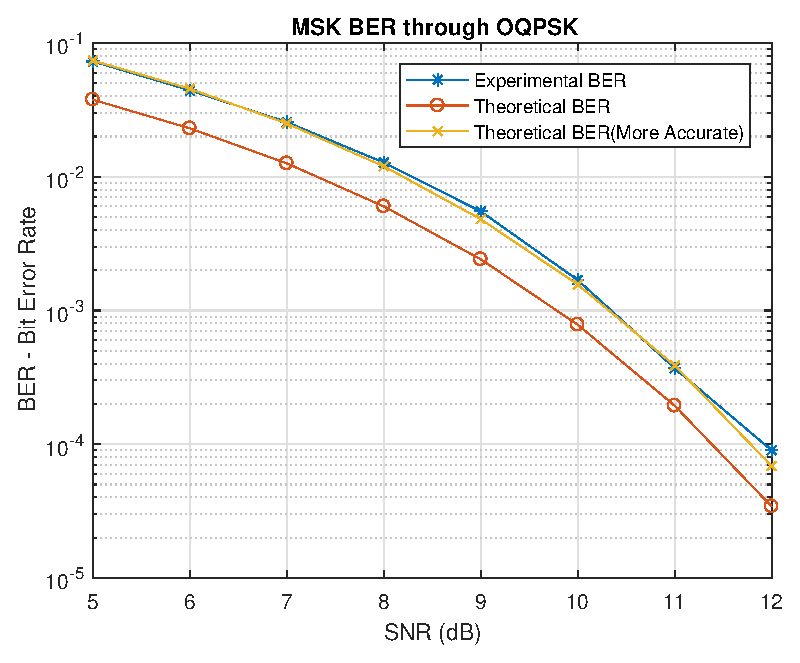
\includegraphics[width=\linewidth]{./results/epsFig}
		\caption{Theoritical vs Experimental without precoding BER}
	\end{subfigure}%
	~
	\begin{subfigure}[t]{0.5\textwidth}
		\centering
		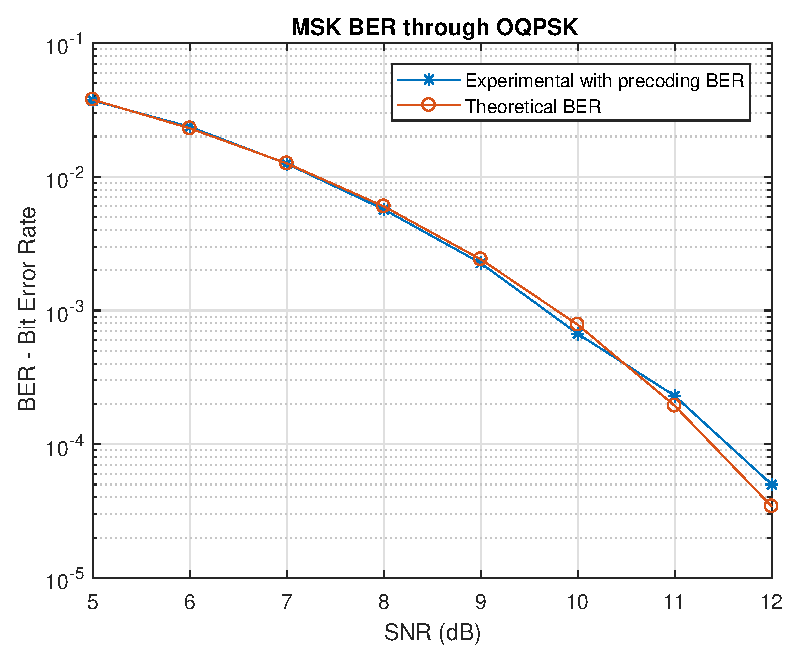
\includegraphics[width=\linewidth]{./results/epsFig1}
		\caption{Theoritical vs Experimental with precoding BER}
	\end{subfigure}
\end{figure}


\end{document}
